% Setup and frequently used packages
\documentclass[12pt]{article}
\usepackage[a4paper, margin=1in]{geometry}
\usepackage[utf8]{inputenc}
\usepackage[T1]{fontenc}
\usepackage{parskip} % Remove indent of new paragraph
\usepackage{titling}
\usepackage{graphicx} % To include graphics such as pictures
\usepackage{amsmath}
\usepackage{caption} % Used to allow empty captions for figures

% Setup title/author/date
\title{Jax Controller Report}
\author{Group 128}
\date{}

% References
\usepackage{hyperref} % Correct formatting for urls in references
\usepackage[style=apa]{biblatex}
\addbibresource{references.bib}

% Header
\usepackage{fancyhdr}
\pagestyle{fancyplain}
\fancyhf{}
\lhead{\theauthor}
\chead{}
\rhead{\thepage}
\renewcommand{\headrulewidth}{0.4pt}
\renewcommand{\plainheadrulewidth}{0.4pt}


\begin{document}
\maketitle

\section*{Bathtub Plant - Classic Controller}

\begin{tabular}{|l|l|}
\hline
\textbf{Parameter}   & \textbf{Value}\\ \hline
Epochs               & 50            \\ \hline
Timesteps            & 50            \\ \hline
Learning Rate        & 0.01          \\ \hline
Disturbance Range    & (-0.05, 0.05) \\ \hline
Initial $K_p$           & 0.1           \\ \hline
Initial $K_i$           & 0.1           \\ \hline
Initial $K_d$           & 0.1           \\ \hline
A                    & 10            \\ \hline
C                    & 0.1           \\ \hline
Initial Height Water & 5             \\ \hline
\end{tabular}

\begin{center}
    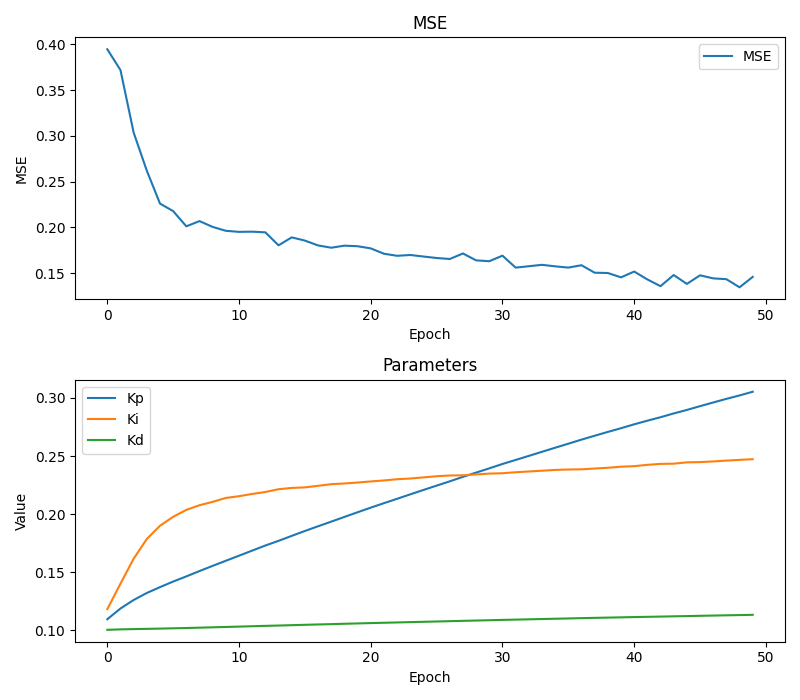
\includegraphics[width=0.8\linewidth]{figures/bathtub-classic.png}
\end{center}

The initial error is not that high but it quickly goes down within the first 10 epochs. After that it continues
to go down, but at a lower rate. Given more epochs it might go down further. The MSE varies but this might be a response
to the relatively high disturbance range. The parameters change more in the earlier epochs, especially the $K_i$. After about
10 epochs the $K_i$ parameter changes at a lower rate. This is probably reflected in the MSE plot after 10 epochs, as we
can see that the rate of change is lower after that point.

\section*{Bathtub Plant - AI Controller}

\begin{tabular}{|l|l|}
    \hline
    \textbf{Parameter}   & \textbf{Value}\\ \hline
    Epochs               & 50            \\ \hline
    Timesteps            & 50            \\ \hline
    Learning Rate        & 0.001          \\ \hline
    Disturbance Range    & (-0.05, 0.05) \\ \hline
    Number of Hidden Layers           & 2           \\ \hline
    Neurons per Layer           & [64, 32]           \\ \hline
    Initial Weight/Bias Range           & (-0.001, 0.001)           \\ \hline
    Activation Function                    & sigmoid            \\ \hline
    A                    & 10           \\ \hline
    C & 0.1             \\ \hline
    Initial Height Water & 5             \\ \hline
\end{tabular}
    
\begin{center}
    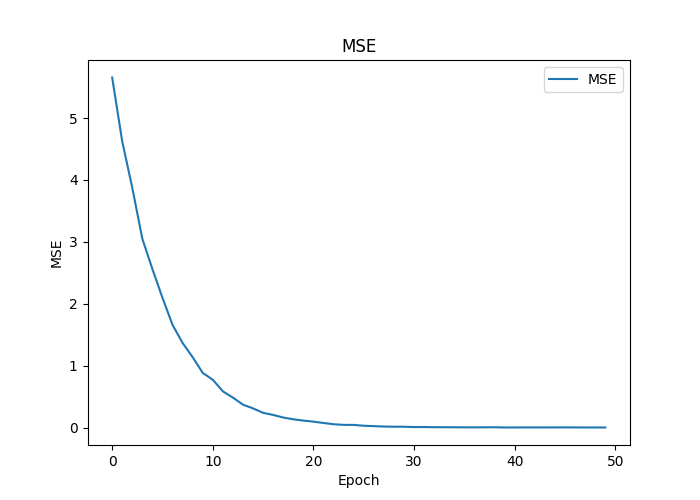
\includegraphics[width=0.8\linewidth]{figures/bathtub-ai.png}
\end{center}

In this run the initial error is higher. This might be because of the random initializing of weights and biases.
We can see that it goes steadily down, but the curve is not that steep. This is because the learning rate in this run is set
to 0.001 instead of 0.01 as in the run with the classic controller above. In particular we observed that the gradients for the
output layer could be high, indicating that these values were far off after initializing them. The controller still manages
to learn, and displays a considerate change in MSE.

\section*{Cournot Plant - Classic Controller}

\begin{tabular}{|l|l|}
    \hline
    \textbf{Parameter}   & \textbf{Value}\\ \hline
    Epochs               & 50            \\ \hline
    Timesteps            & 50            \\ \hline
    Learning Rate        & 0.01          \\ \hline
    Disturbance Range    & (-0.05, 0.05) \\ \hline
    Initial $K_p$           & 0.1           \\ \hline
    Initial $K_i$           & 0.1           \\ \hline
    Initial $K_d$           & 0.1           \\ \hline
    A                    & 10            \\ \hline
    C                    & 0.1           \\ \hline
    Initial Height Water & 5             \\ \hline
\end{tabular}

\begin{center}
    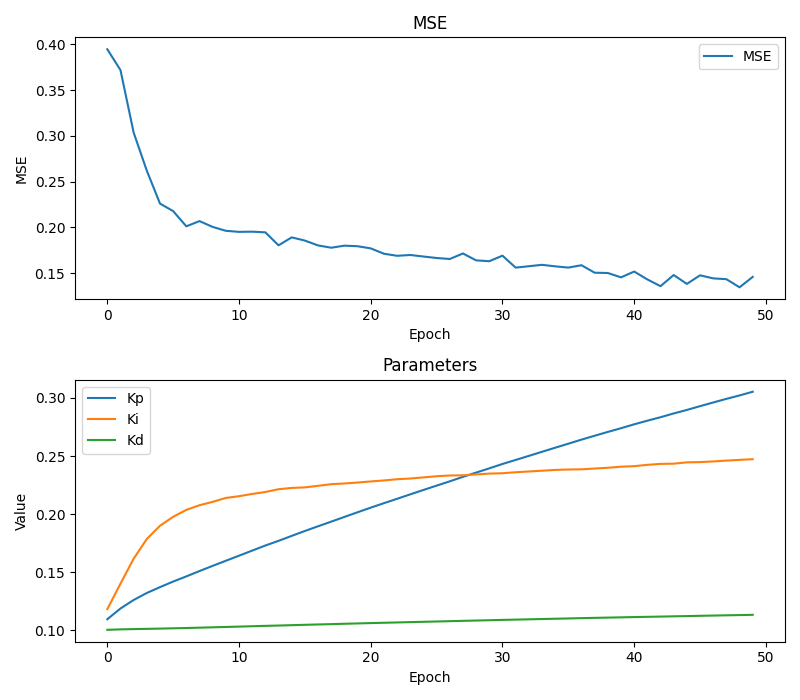
\includegraphics[width=0.8\linewidth]{figures/bathtub-classic.png}
\end{center}

The initial error is not that high but it quickly goes down within the first 10 epochs. After that it continues
to go down, but at a lower rate. Given more epochs it might go down further. The MSE varies but this might be a response
to the relatively high disturbance range. The parameters change more in the earlier epochs, especially the $K_i$. After about
10 epochs the $K_i$ parameter changes at a lower rate. This is probably reflected in the MSE plot after 10 epochs, as we
can see that the rate of change is lower after that point.

\section*{Cournot Plant - AI Controller}

\section*{Population Plant - Classic Controller}

\section*{Population Plant - AI Controller}




\begin{verbatim}
Training set MSE: 0.0392
Test set MSE: 0.0399
\end{verbatim}

The result above was obtained with a learning rate of 0.001 and 1000 epochs. 

\begin{verbatim}
Training set MSE: 0.0504
Test set MSE: 0.0517
\end{verbatim}

The result above was obtained after setting the amount of epochs to 100 instead of 1000. Still using a learning rate of 0.001.

\begin{verbatim}
Training set MSE: 0.0389
Test set MSE: 0.0383
\end{verbatim}

The best results was obtained with a learning rate of 0.05 and 1000 epochs. Slightly better than a learning rate of
0.001

\section*{Population Plant Description}

This plant is based on Lotka-Volterra equations that say something about the oscilation of population
in ecologic systems.



\printbibliography

\end{document}